\documentclass[12pt]{report}
\usepackage{graphicx}
\usepackage{subfigure}
\usepackage{url}
\usepackage{color}
\usepackage{fullpage}
%\usepackage{geometry} % see geometry.pdf on how to lay out the page. There's lots.
%\geometry{letterpaper} % or letter or a5paper or ... etc
% \geometry{landscape} % rotated page geometry

% See the ``Article customise'' template for come common customisations

\title{HPS SVT Maintenance Manual \\ v1.0}
\author{Authors: \\
Per Hansson, John Jaros, Takashi Maruyama, Omar Moreno,\\ Tim Nelson, Marco Oriunno, Sho Uemura\footnote{contact person for this document}}
\date{June 10, 2015} % delete this line to display the current date

%%% BEGIN DOCUMENT
\begin{document}

\maketitle

Between run periods, both the SVT chiller (big Julabo chiller, HFE-7000 fluid) and the FEB chiller (small Anova chiller, distilled water) are kept running.

The silicon needs to be kept cool to prevent reverse annealing, so an SVT chiller outage of more than a couple of days is cause for concern. The FEB chiller is not so important (only needs to be running during DAQ tests).

The SVT chiller needs to be topped off with additional fluid every 3 weeks. When the chiller level (check the screen, visible on cctv7) reaches level 2 (see figure \ref{fig:svt_chiller_level}), follow the procedure in section \ref{sec:proc_svt_chiller_refill}.

Between run periods, the normal setpoint for the SVT chiller is 17 C. This keeps the SVT above dew point, so it is not necessary to maintain vacuum/dry gas on the SVT. 
The SLAC group may want the SVT cold for a week or two so the hybrids can be powered; the SVT needs to be under vacuum to prevent condensation. Follow the procedure in section \ref{sec:proc_svt_chiller_tempchange} to change the setpoint.

\begin{table}[h]
\begin{center}
\begin{tabular}{|l|l|l|}
\hline
Parameter & Normal & SVT cold \\
\hline
SVT chiller setpoint (C) & 17 & -20 \\
SVT supply RTD alarms (C) & 15/16/19/20 & -22/-21/-17/-16 \\
SVT return RTD alarms (C) & 15/16/19/20 & -22/-21/-17/-16 \\
FEB chiller setpoint (C) & 20 & 20 \\
\hline
\end{tabular}
\end{center}
\caption{SVT cooling settings between run periods.}
\end{table}

\section{Contact List}

Contact Sho Uemura (646-833-8746, {\url{meeg@slac.stanford.edu}, \url{uemura@jlab.org}}). If not reachable, contact Pelle Hansson (650-391-6233, \url{phansson@slac.stanford.edu}, \url{phansson@jlab.org}).

\begin{center}
    \begin{tabular}{lc}
        \hline \hline 
        System & Experts \\
        \hline
        General expert & Tim Nelson \\
        SVT DAQ & Pelle Hansson \\
        SVT EPICS controls & Pelle Hansson, Wesley Moore \\
        MPOD power supply & Sho Uemura \\
        PLC interlocks & Brian Eng \\
        Cooling & Sho Uemura \\
        \hline \hline
    \end{tabular}
\end{center}

\chapter{Controls and monitoring}

\section{SVT Cooling}

All the GUIs shown below are accessed through the \textbf{Devices} menu in \textbf{hps\_epics}. Chiller and interlock settings should only be modified under the supervision of an SVT Expert. Table~\ref{tab:cooling_settings} lists the default settings for the SVT and FEB chillers and alarms during running (cold) and between runs when the beam enclosure is open for servicing (warm).

\begin{figure*}[!ht]
    \begin{center}
        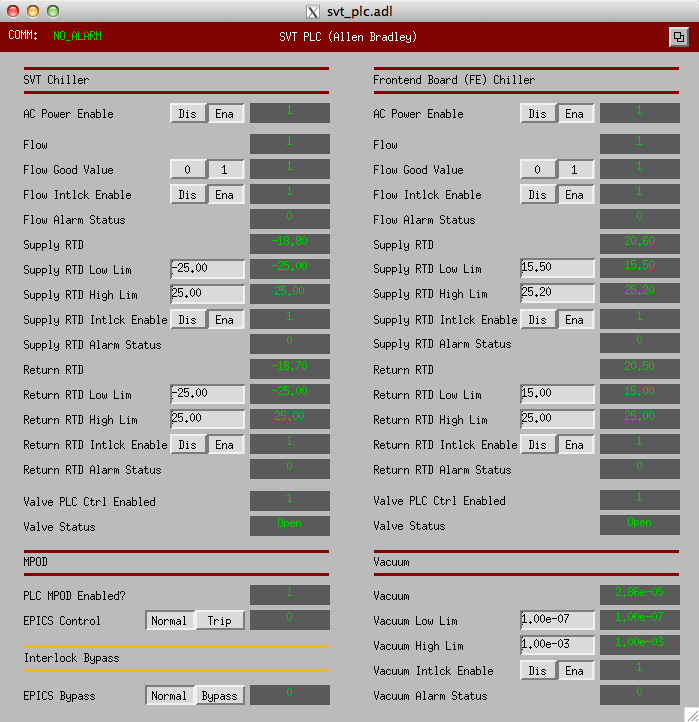
\includegraphics[width=0.5\textwidth]{svt_plc.png}
        \caption{SVT PLC GUI, accessed through the \textbf{Devices} menu in \textbf{hps\_epics}.}
        \label{fig:ctrl_cooling_plc}
    \end{center}
\end{figure*}

\begin{figure*}[!ht]
    \begin{center}
        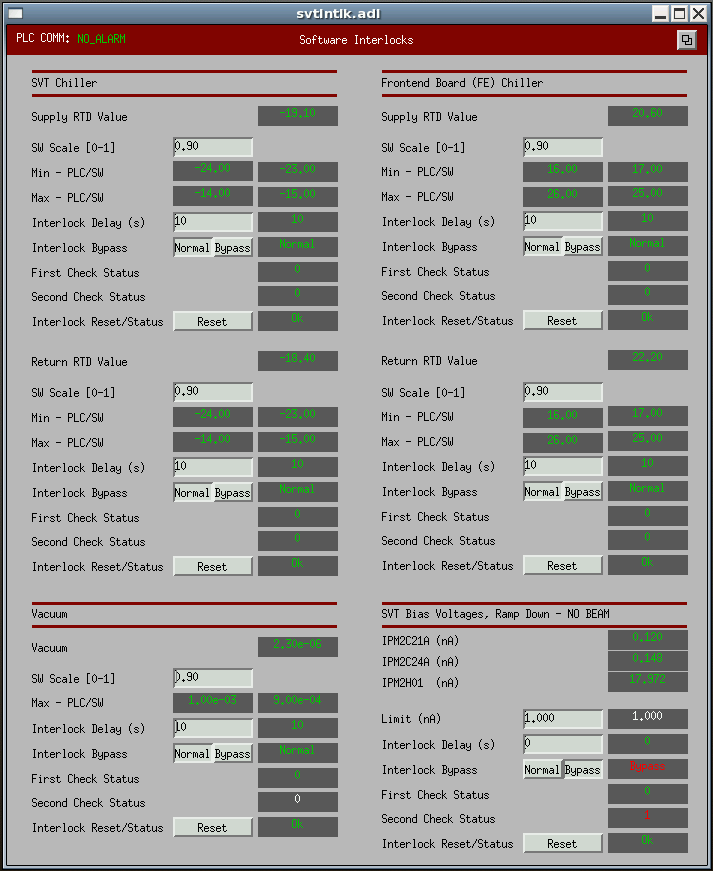
\includegraphics[width=0.4\textwidth]{svt_softinterlocks.png}
        \caption{SVT software interlocks GUI, accessed through the \textbf{Devices} menu in \textbf{hps\_epics}.}
        \label{fig:ctrl_cooling_softinterlocks}
    \end{center}
\end{figure*}

\begin{figure*}[!ht]
    \begin{center}
        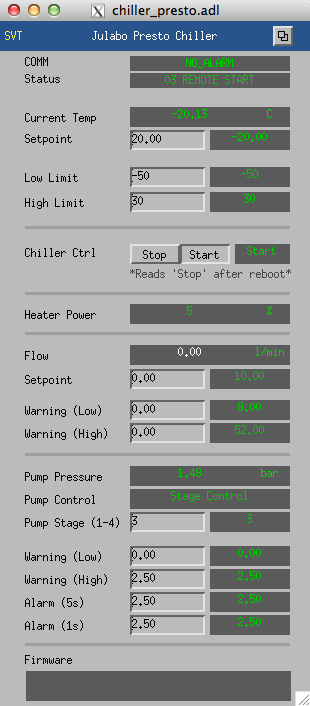
\includegraphics[width=4cm]{figures/svt_svtChiller.png}
        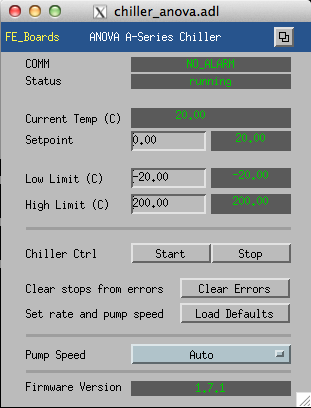
\includegraphics[width=0.3\textwidth]{figures/svt_febChiller.png}
        \caption{SVT (left) and FEB (right) chiller GUIs, accessed through the \textbf{Devices} menu in \textbf{hps\_epics}.}
        \label{fig:ctrl_cooling_chillers}
    \end{center}
\end{figure*}

\begin{table}[h]
\begin{center}
\begin{tabular}{|l|l|l|}
\hline
Parameter & SVT warm & SVT cold \\
\hline
SVT chiller setpoint ($^\circ$C) & 17 & -20 \\
SVT RTD alarms (\textbf{{\color{red} low}/{\color{yellow} low}/{\color{yellow}high}/{\color{red}high}}) ($^\circ$C) & \textbf{{\color{red}15}/{\color{yellow}16}/{\color{yellow}18}/{\color{red}19}} & \textbf{{\color{red}-22}/{\color{yellow}-21}/{\color{yellow}-17}/{\color{red}-16}} \\
SVT RTD PLC limits ($^\circ$C) & bypassed & -24/-14 \\
FEB chiller setpoint ($^\circ$C) & 20 & 20 \\
FEB RTD alarms (\textbf{{\color{red} low}/{\color{yellow} low}/{\color{yellow}high}/{\color{red}high}}) ($^\circ$C) & \textbf{{\color{red}16}/{\color{yellow}17}/{\color{yellow}25}/{\color{red}26}} & \textbf{{\color{red}16}/{\color{yellow}17}/{\color{yellow}25}/{\color{red}26}} \\
FEB RTD PLC limits ($^\circ$C) & bypassed & 16/26 \\
\hline
\end{tabular}
\end{center}
\caption{Default SVT cooling settings.  Minor alarm limits are in yellow and major alarm limits are in red.}
\label{tab:cooling_settings} 
\end{table}

Any major (red) ALH alarm under the ``SVT/COOLING'' group will send an e-mail alert. Also, there is a webcam (cctv7) pointed at the SVT chiller screen. The webcam can be set to e-mail a snapshot every 24 hours. 

\chapter{Procedures}

\section{Cooling and Interlocks}
\label{sec:proc_cooling}
\subsection{Start FEB chiller}
\begin{enumerate}
    \item Disable the PLC interlock for FEB flow (PLC GUI, upper right).
    \item Verify that the chiller temperature setpoint is 20 C. If not, call the SVT expert.
    \item Check the RTD temperature limits. The low limits should be set at 16 C and the high limits at 26 C.
    \item Verify that all PLC alarms that affect the FEB chiller loop (supply RTD, return RTD, and vacuum) are in ``0'' state.
    \item Verify that the FEB valve is open.
    \item Start the chiller.
    \item Wait for the flow switch value to change, then enable the FEB flow interlock.
        If the flow switch does not trigger, call the SVT expert.
    \item At this point, the FEBs can be powered.
    \item The \textbf{current temperature} shown in the FEB chiller GUI should converge to the setpoint in a few minutes.
    \item When the temperature has reached the setpoint, lower the high limits in the interlock to their final values.
\end{enumerate}

\subsection{Start SVT chiller}
\begin{enumerate}
    \item Change the chiller temperature setpoint to 17 C. (This assumes the SVT cooling loop is at room temperature to start. If it is cold, start cold.)
    \item Disable the PLC interlocks for SVT flow, supply RTD, and return RTD (left side of PLC GUI).
        Disable the software interlocks for supply RTD and return RTD (left side of software interlock GUI).
        Verify all PLC alarms and software interlocks are in ``Ok'' or ``0'' state, and the SVT valve is open (PLC GUI).
    \item Start the chiller.
    \item Wait for the flow switch value to change, then enable the SVT flow interlock.
    \item Wait for the chiller temperature to stabilize at the setpoint.
        Some oscillation is normal in the short term, and the chiller may trip off (most likely if the chiller has been off for a while).
        If this happens, power cycle the chiller (power switch to the left of the touch screen, or ``AC Power Enable'' on the PLC GUI), and start over from the beginning of the procedure.
    \item Follow the procedure in section \ref{sec:proc_svt_chiller_tempchange} to change the temperature to its desired value.
\end{enumerate}

\subsection{Stop FEB chiller}
\begin{enumerate}
    \item Verify that hybrid bias, FEB power, and flange board power are off.
    \item Press the \textbf{Stop} button in the FEB chiller GUI. The interlocks will close the FEB valve and trip the MPOD.
\end{enumerate}

\subsection{Stop SVT chiller}
\begin{enumerate}
    \item Verify that hybrid bias, FEB power, and flange board power are off.
    \item Press the \textbf{Stop} button in the SVT chiller GUI. The interlocks will close the SVT valve and trip the MPOD.
\end{enumerate}

\subsection{Draining SVT chiller (experts only)}
\begin{enumerate}
    \item Disable the PLC interlocks for SVT chiller flow, supply RTD, and return RTD (left side of PLC GUI).
    \item Put the chiller in manual mode using the touchscreen.
    \item Follow the instructions in the chiller manual to drain the chiller. Use the big plastic jug and the two short pieces of rubber tube.

    \item When you disconnect a fitting in the chiller loop, drain both connections into a beaker.
    \item Purge both connections using the nitrogen line (use a Swagelok-to-VCR adapter with a used gasket), with the reservoir drain valve (the ball valve with a plastic handle) open.
        Be sure to cap the connection not being purged using a VCR cap and a used gasket. 
\end{enumerate}

\subsection{Filling SVT chiller from empty (experts only)}
\begin{enumerate}
    \item Disable the PLC interlocks for SVT chiller flow, supply RTD, and return RTD (left side of PLC GUI).
    \item Follow the instructions in the chiller manual to fill the chiller. Use the metal funnel.
    \item If the final level of the chiller is below 1/4, add a full jug of HFE 7000.
\end{enumerate}

\subsection{Changing SVT chiller temperature}
\label{sec:proc_svt_chiller_tempchange}
\begin{enumerate}
    \item Disable the PLC and software interlocks for SVT chiller supply RTD and return RTD (these are left disabled between run periods).
    \item Change the setpoint on the SVT chiller GUI in steps of no more than 10 degrees C.
        After each step, wait 20 minutes for temperatures to equalize in the system (chiller temperature and RTDs should stabilize in about 10 minutes).
        Check cooling lines for frost or melting ice.
    \item When at final temperature, set the alarm and interlock setpoints for the SVT chiller supply RTD and return RTD.
        Re-enable interlocks if they were bypassed.
\end{enumerate}

\subsection{Adding fluid to SVT chiller}
\label{sec:proc_svt_chiller_refill}
The HFE-7000 fluid for the SVT cooling loop evaporates steadily and must be replenished approximately once every 3 weeks.
The fluid is supplied in 10-pound jugs. It is nontoxic and evaporates rapidly, so don't worry about small spills.
The chiller should be refilled when it reaches level 2 (slightly below 1/4); one jug will take it to level 7 (slightly above 3/4).
Refilling before the level drops to level 2 will cause a high level warning; waiting until the level drops to level 1 will cause a low level warning.

It is safe to add fluid while the chiller is running. This may cause a temperature spike, so RTD interlocks must be disabled.

\begin{enumerate}
    \item Disable the PLC and software interlocks for SVT chiller supply RTD and return RTD (these are left disabled between run periods).
    \item Using a funnel, pour a jug of HFE-7000 into the fill port at the top of the chiller (open the metal cover and pull out the white plastic plug). If this causes a high level warning, acknowledge it.
    \item Wait 5 minutes or until temperatures have stabilized (can use the stripchart on the chiller's touchscreen).
    \item Check the water level in the FEB chiller (minimum: the cooling coil should be covered, maximum: 1.5 inches below the rim).
    \item Check that none of the temperatures are alarming (RTD values in the interlock GUIs should be green). Enable all interlocks that were bypassed.
    \item Make a logbook entry noting the chiller level before and after the fill, and the number of full HFE jugs remaining.
\end{enumerate}

\begin{figure}
    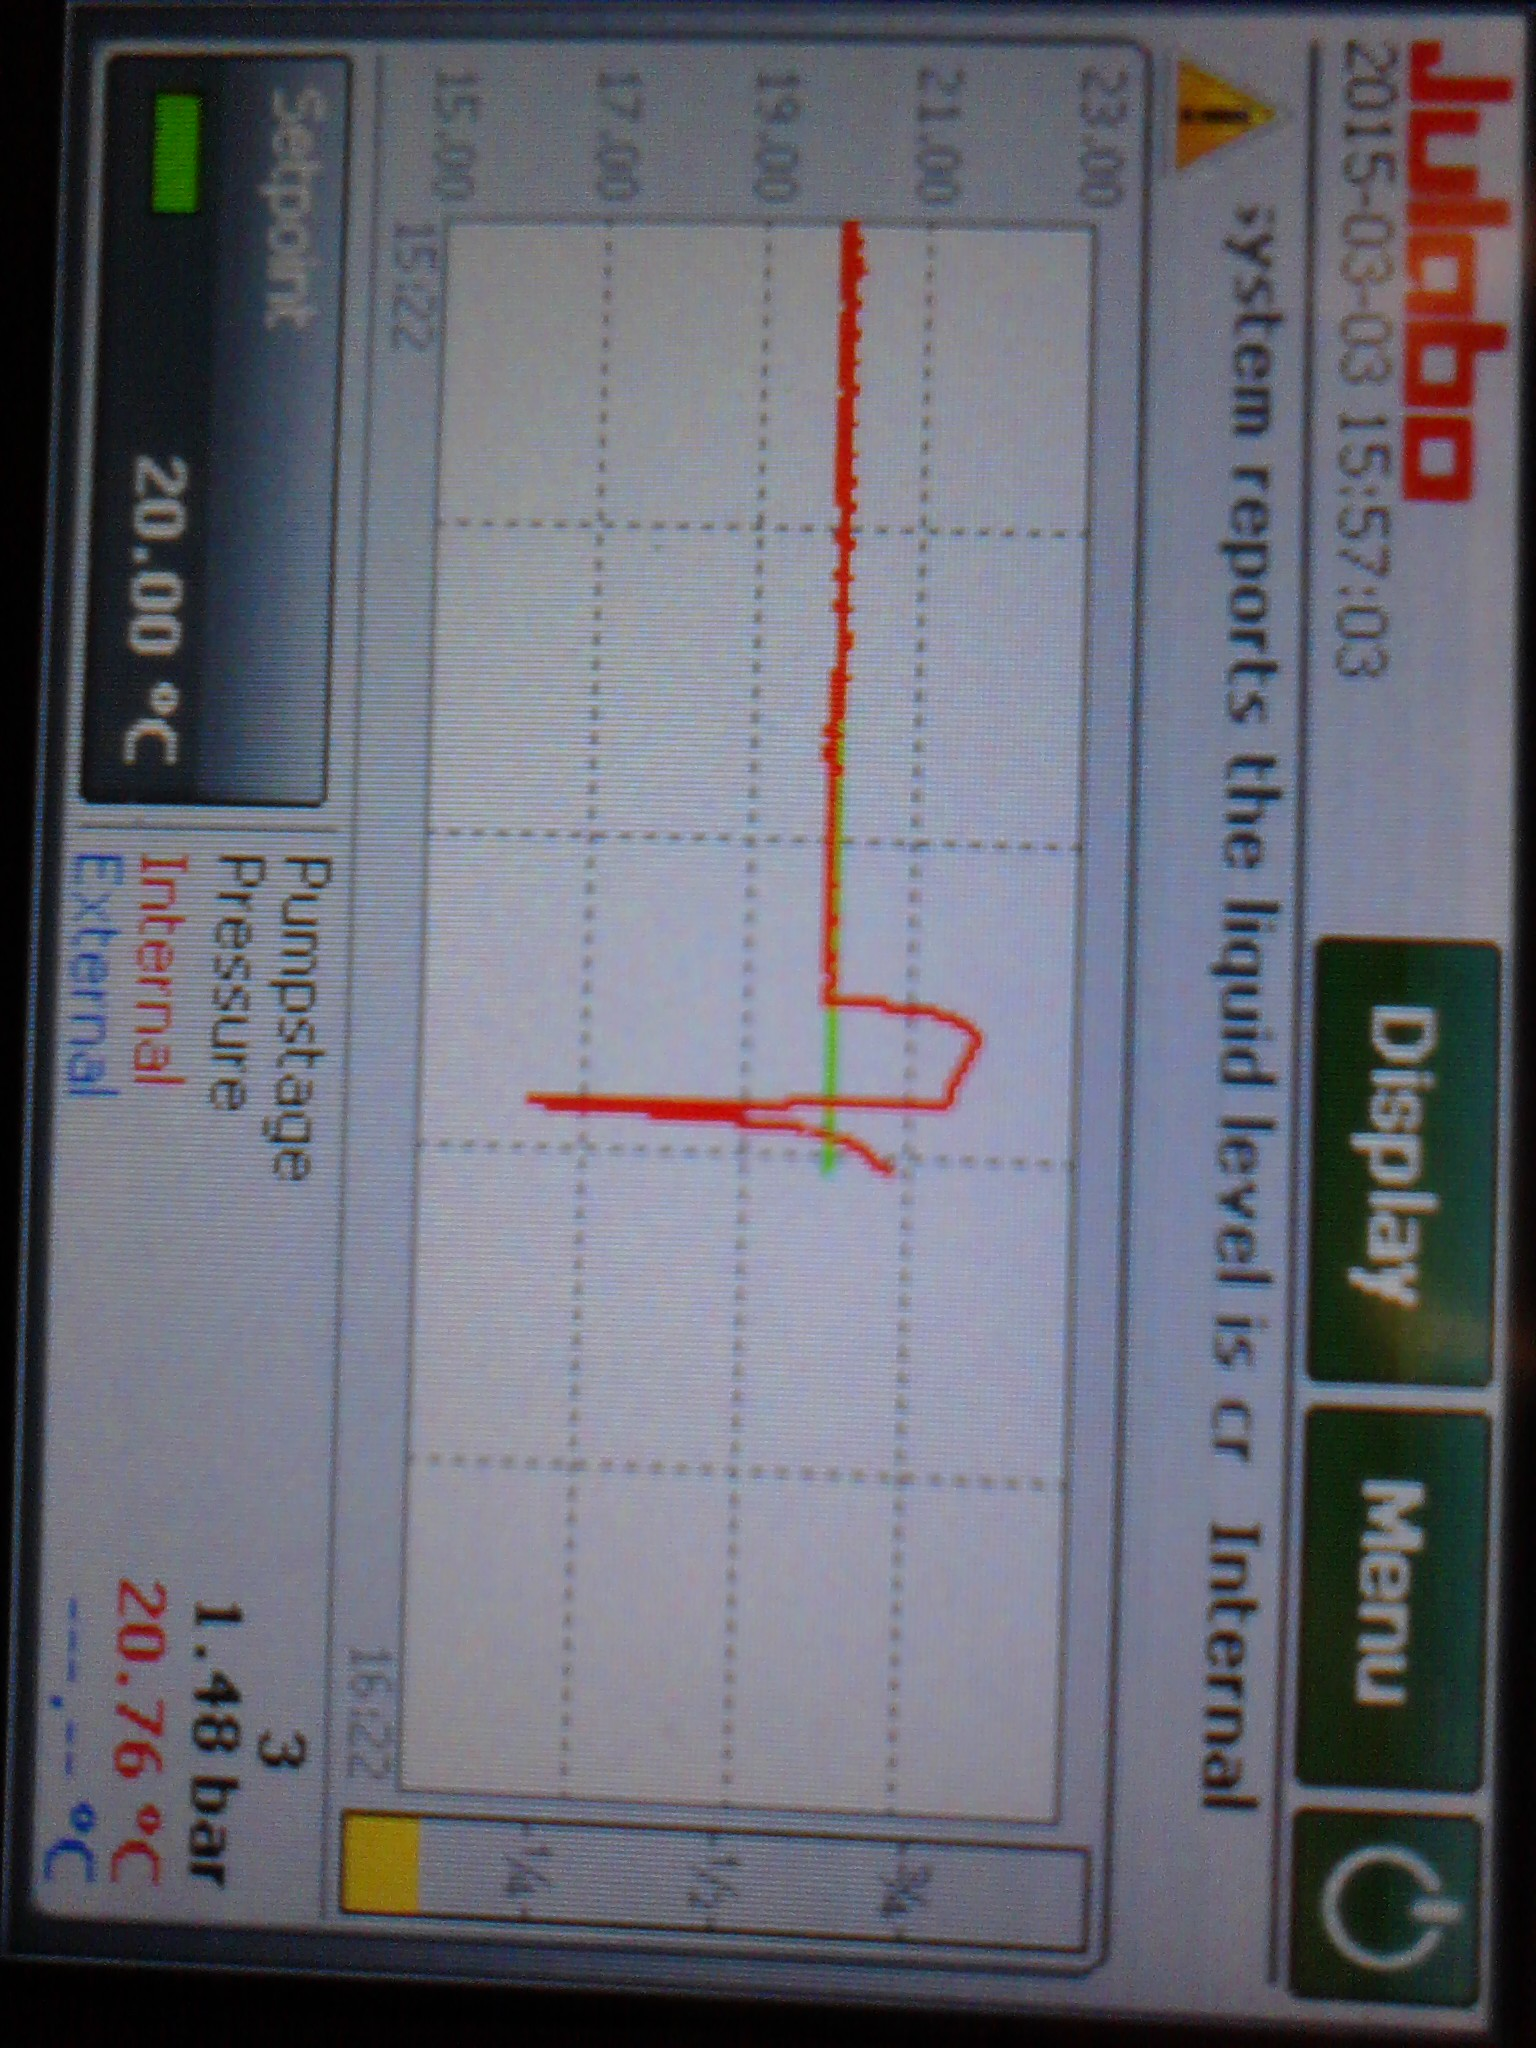
\includegraphics[angle=90,width=6cm]{figures/chiller_level1}
    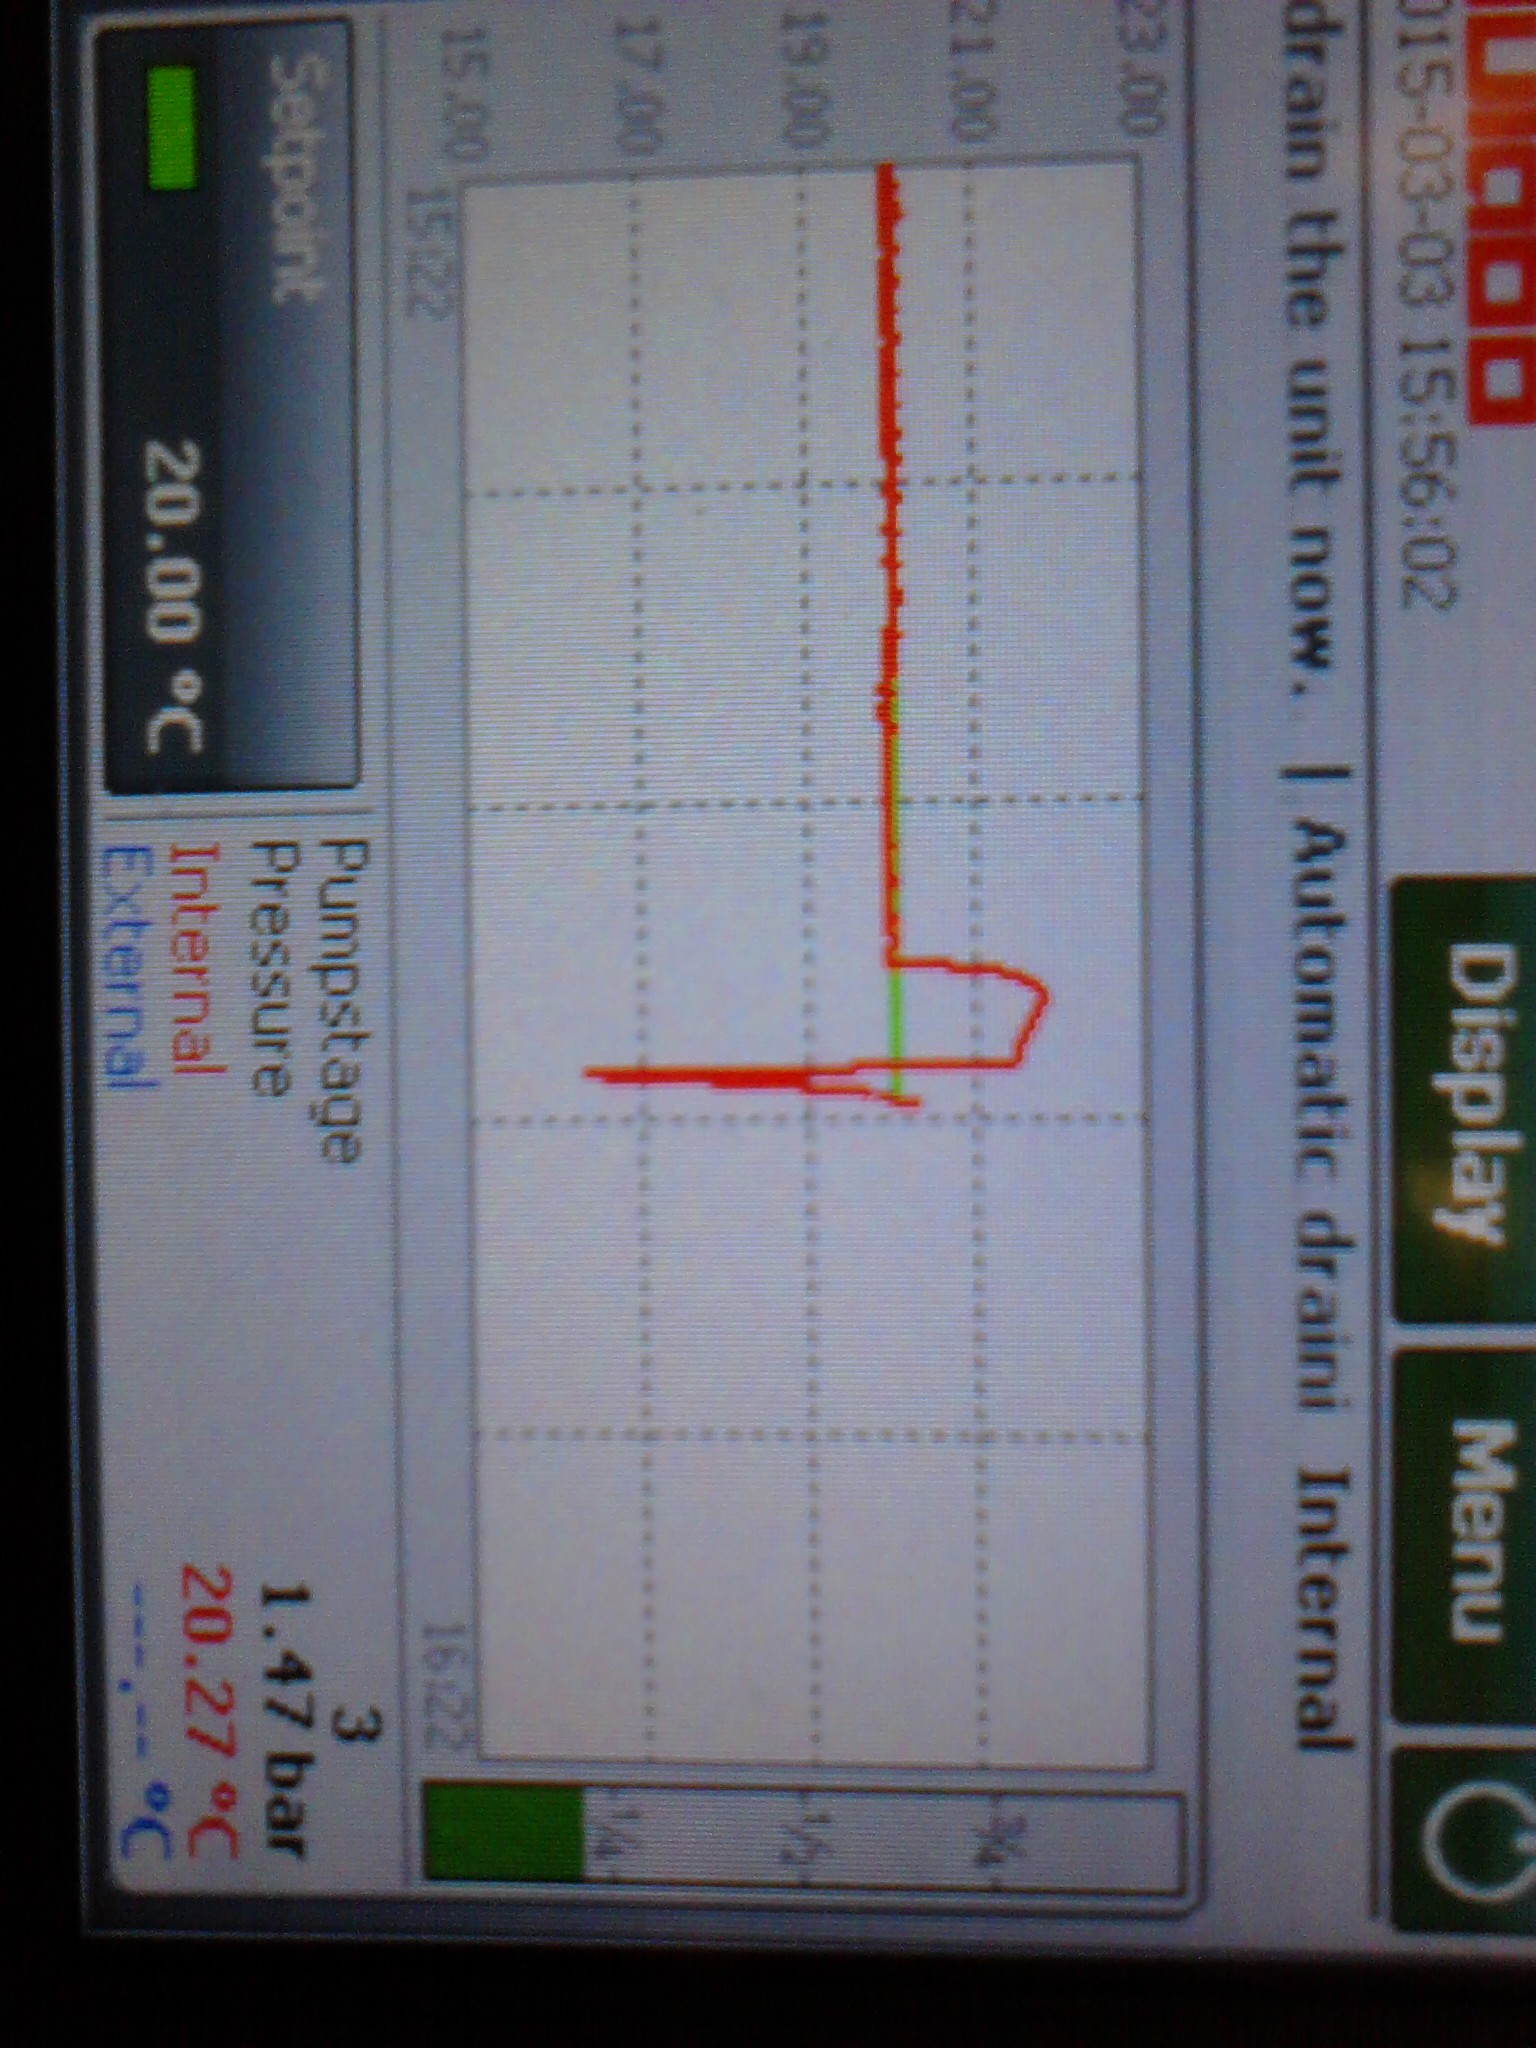
\includegraphics[angle=90,width=6cm]{figures/chiller_level2}
    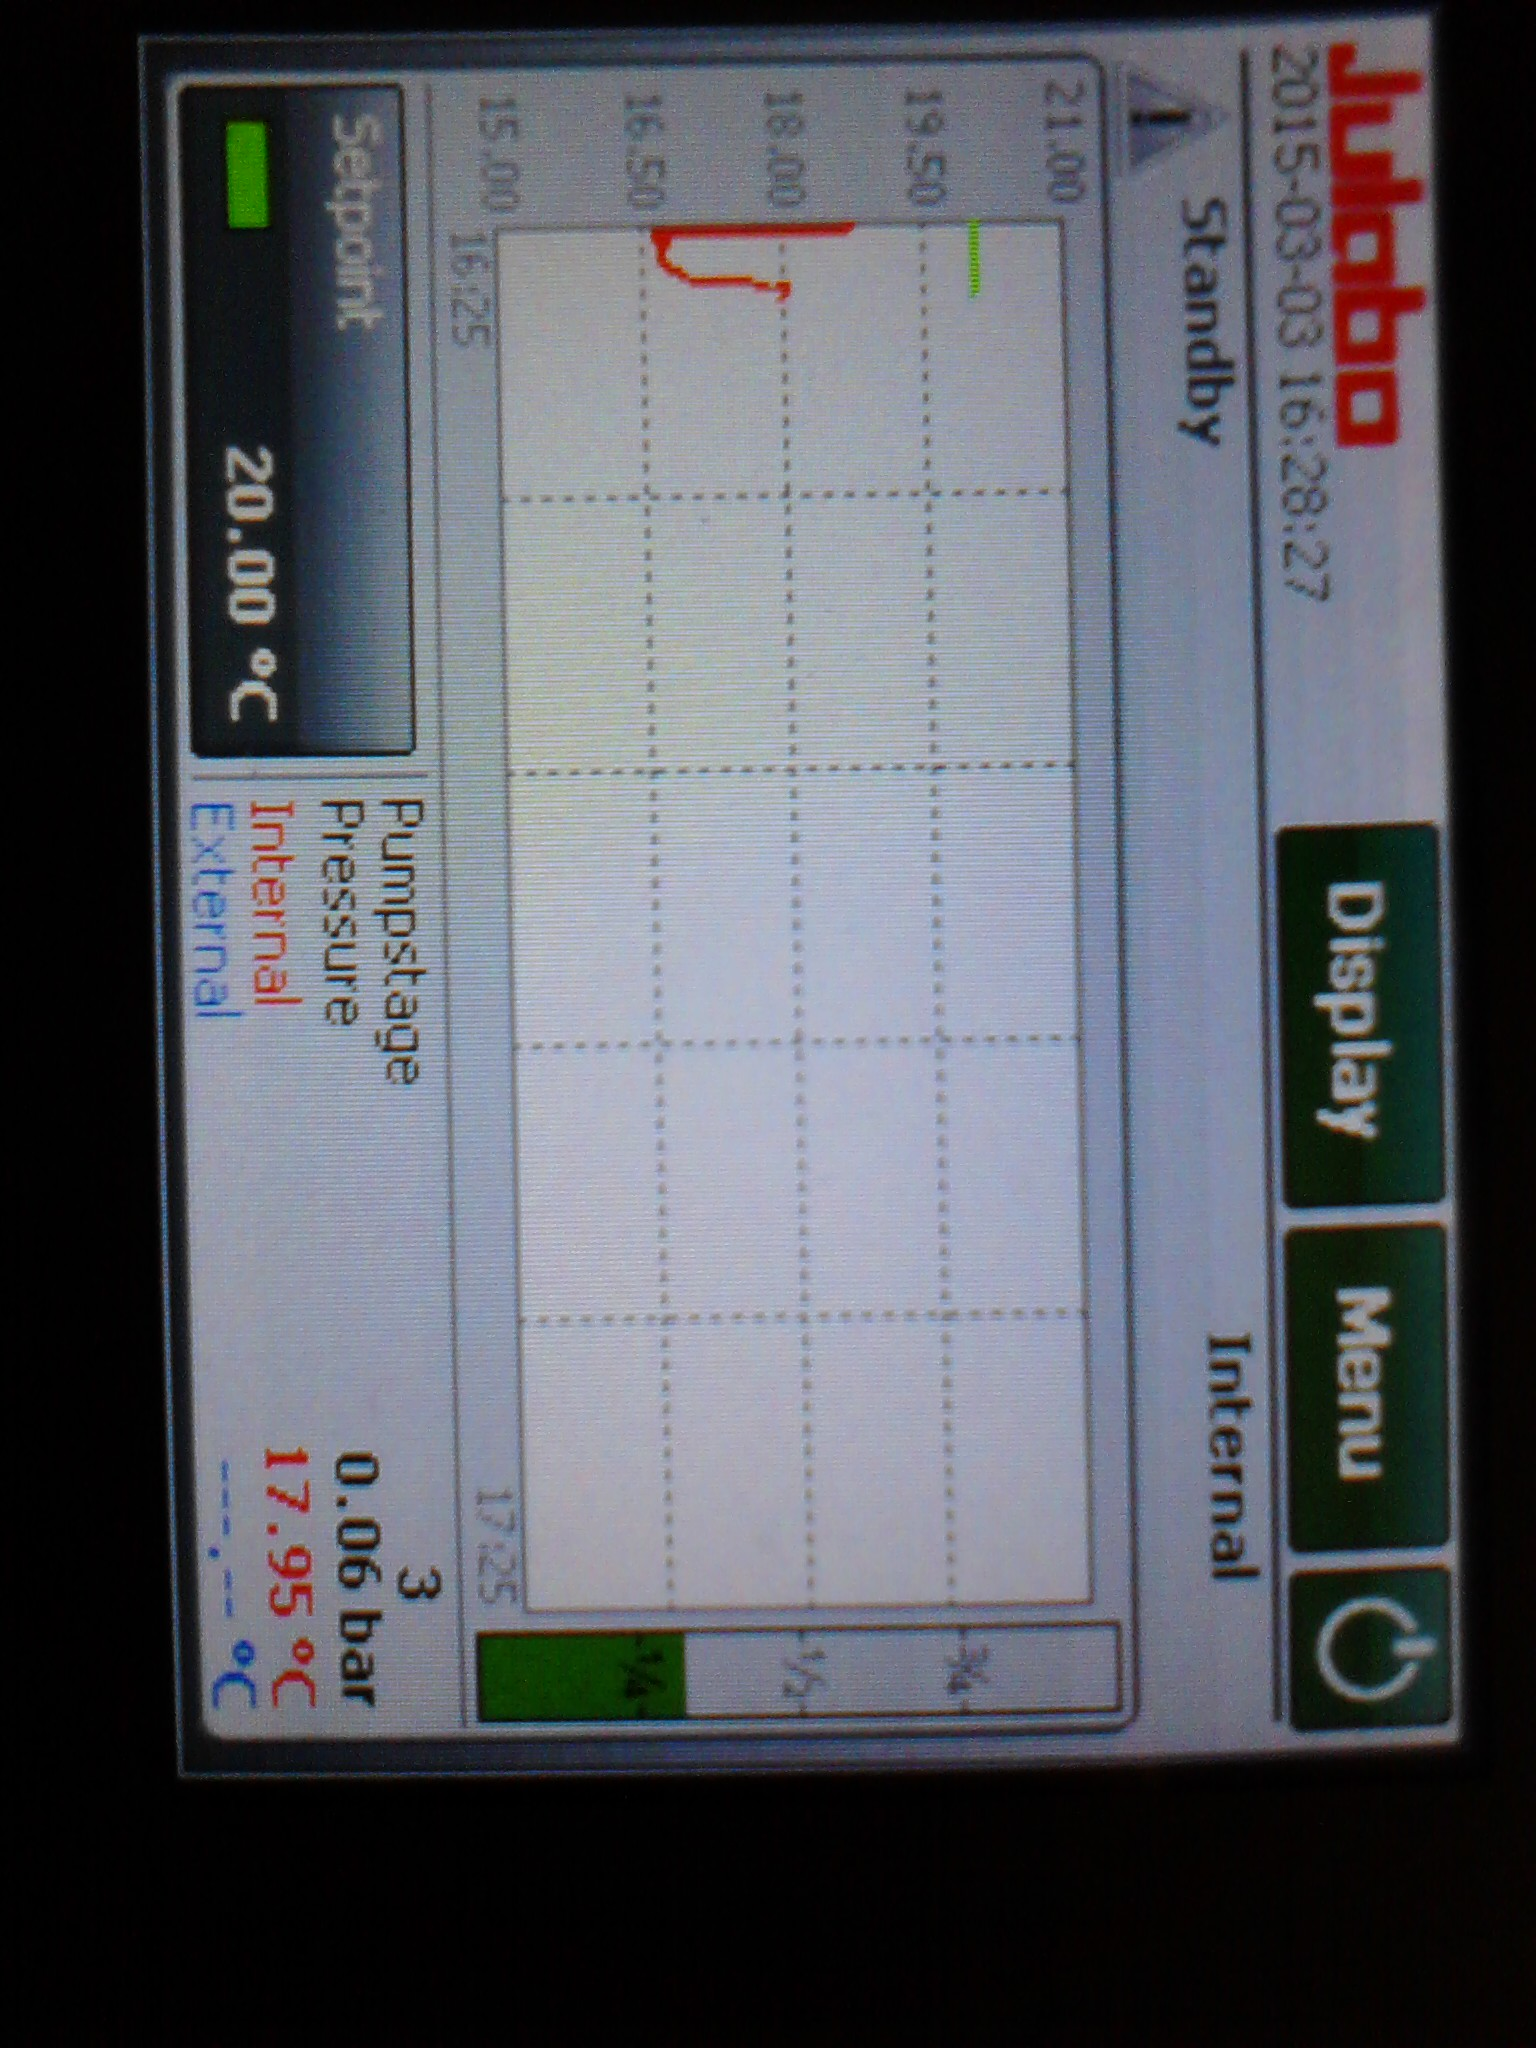
\includegraphics[angle=90,width=6cm]{figures/chiller_level3}
    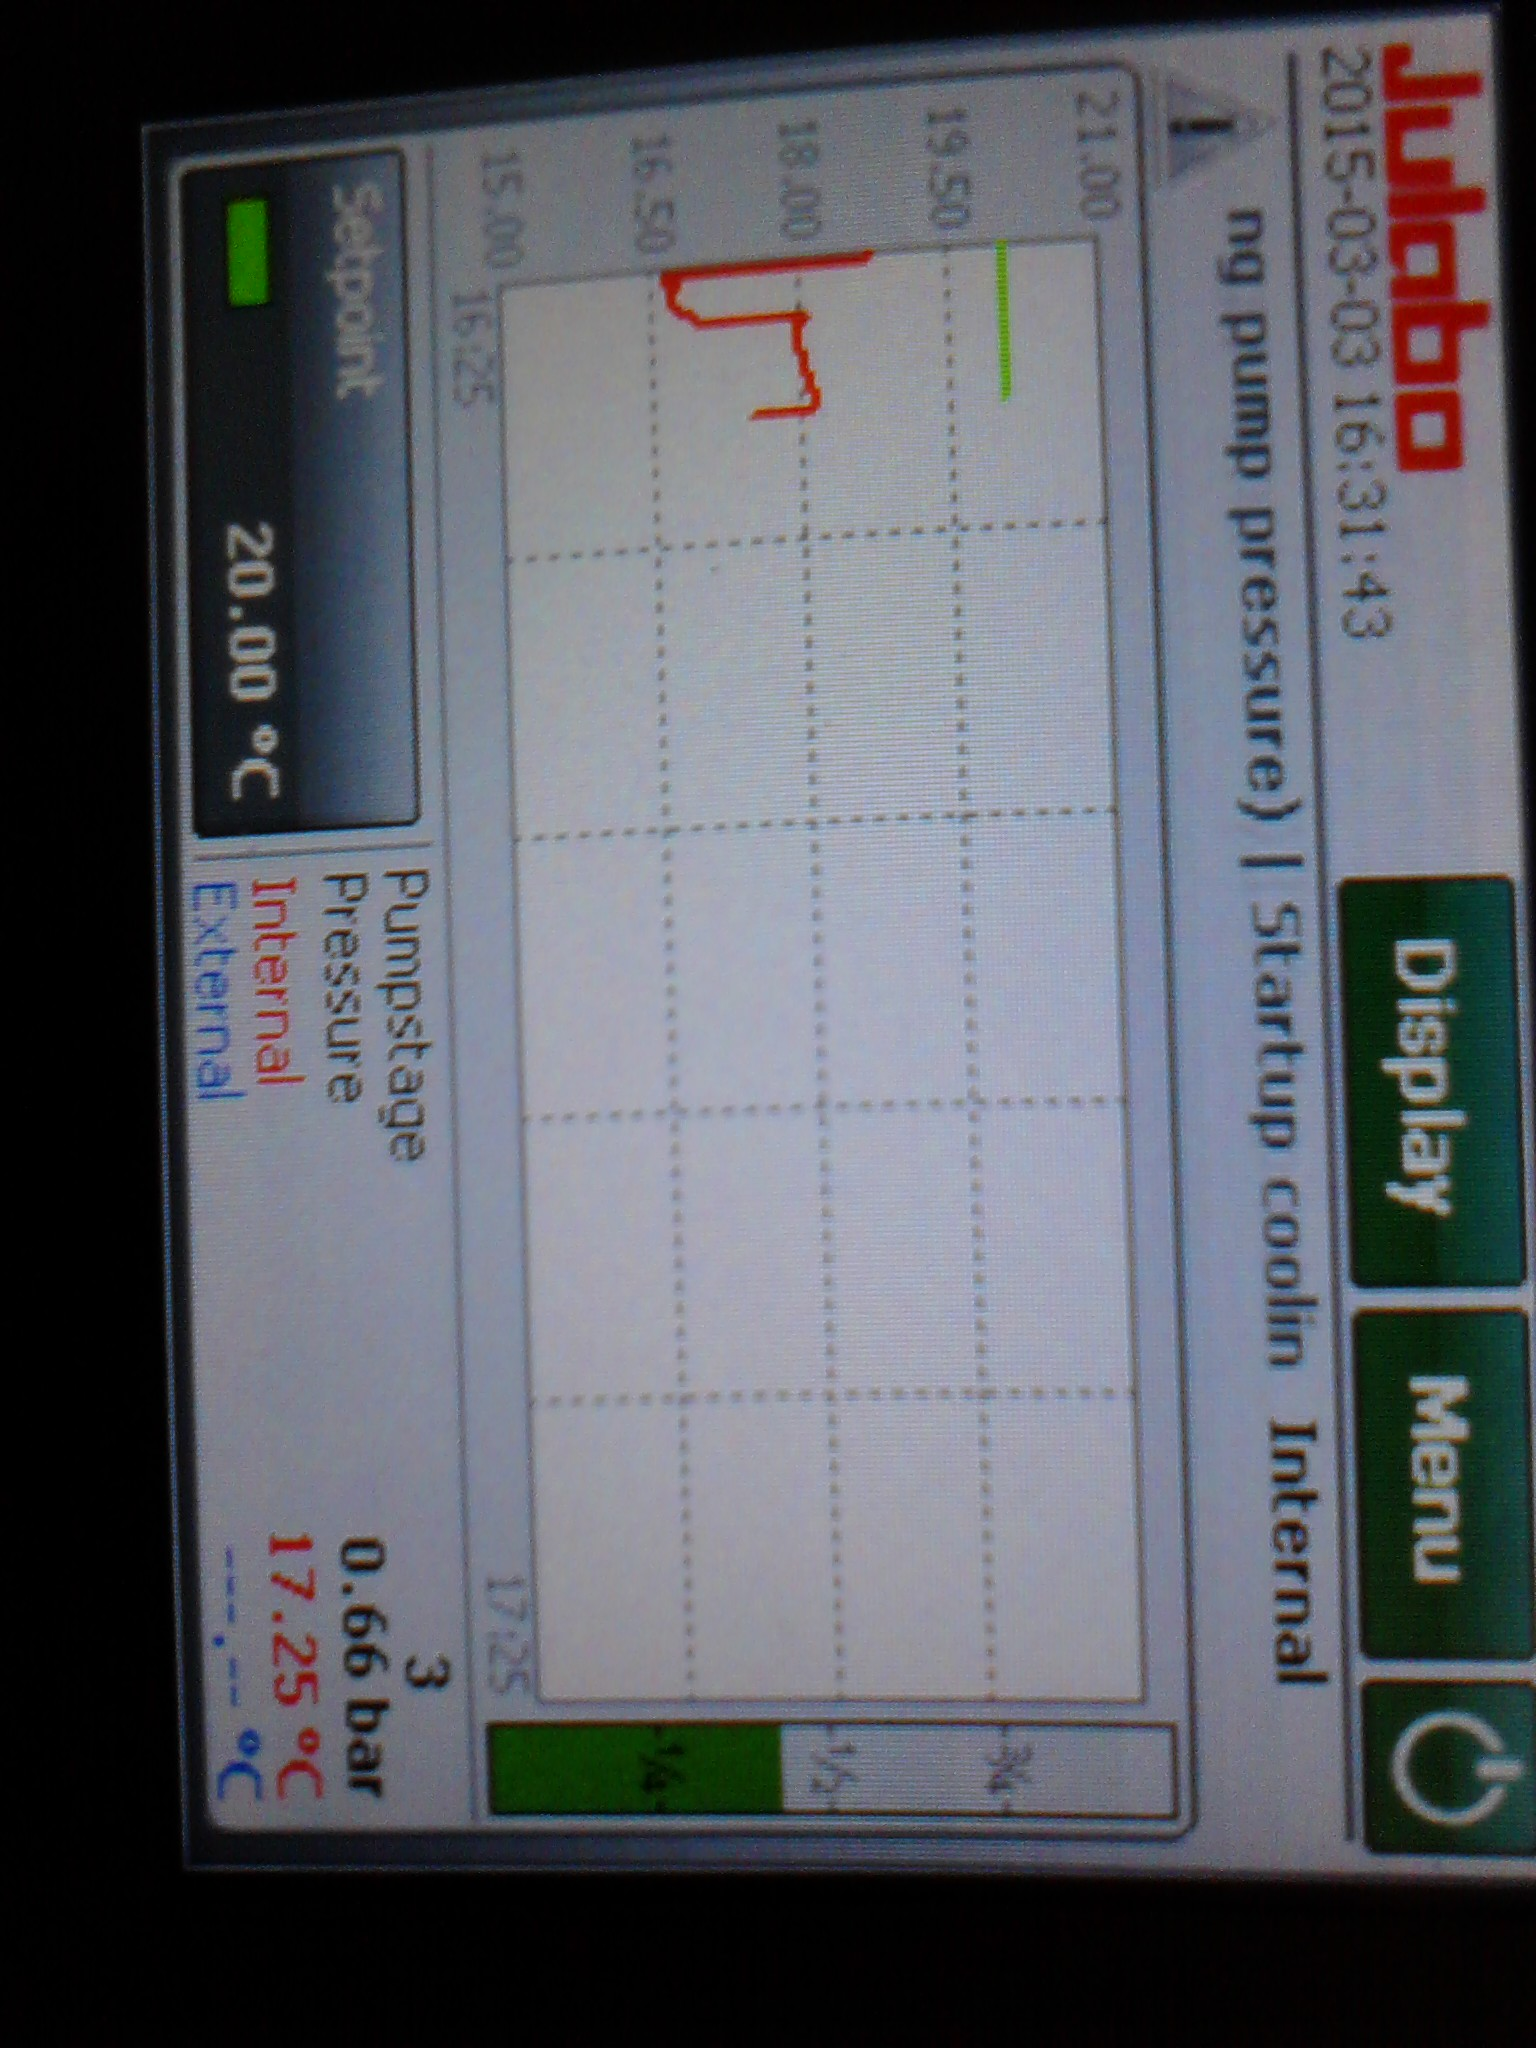
\includegraphics[angle=90,width=6cm]{figures/chiller_level4}
    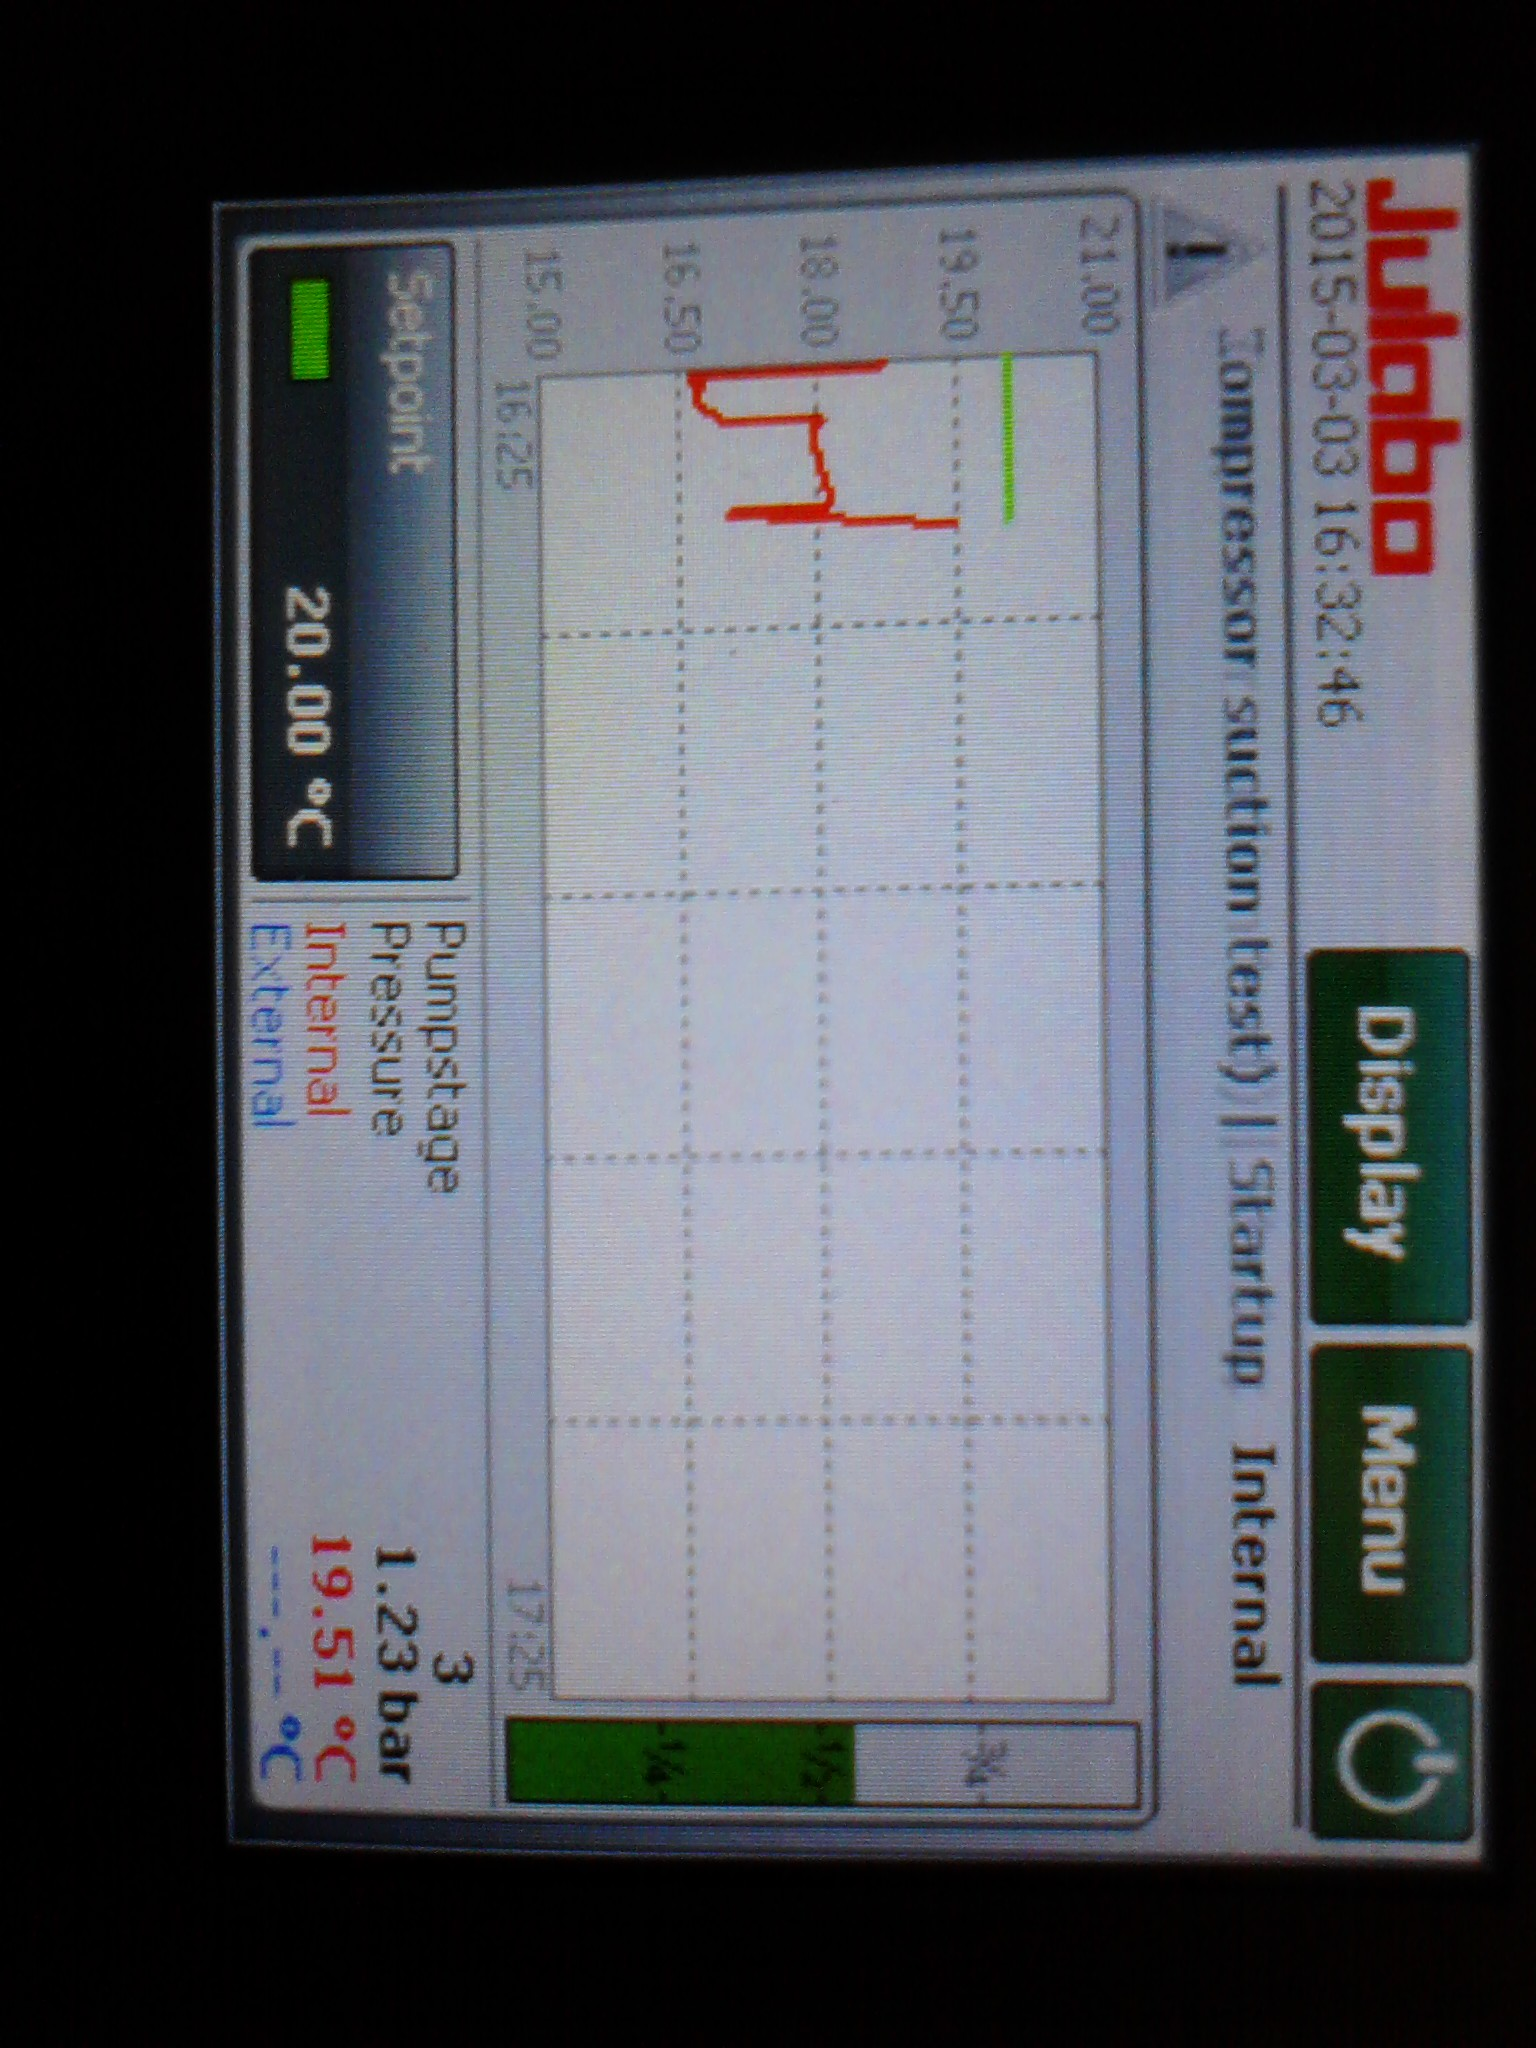
\includegraphics[angle=90,width=6cm]{figures/chiller_level5}
    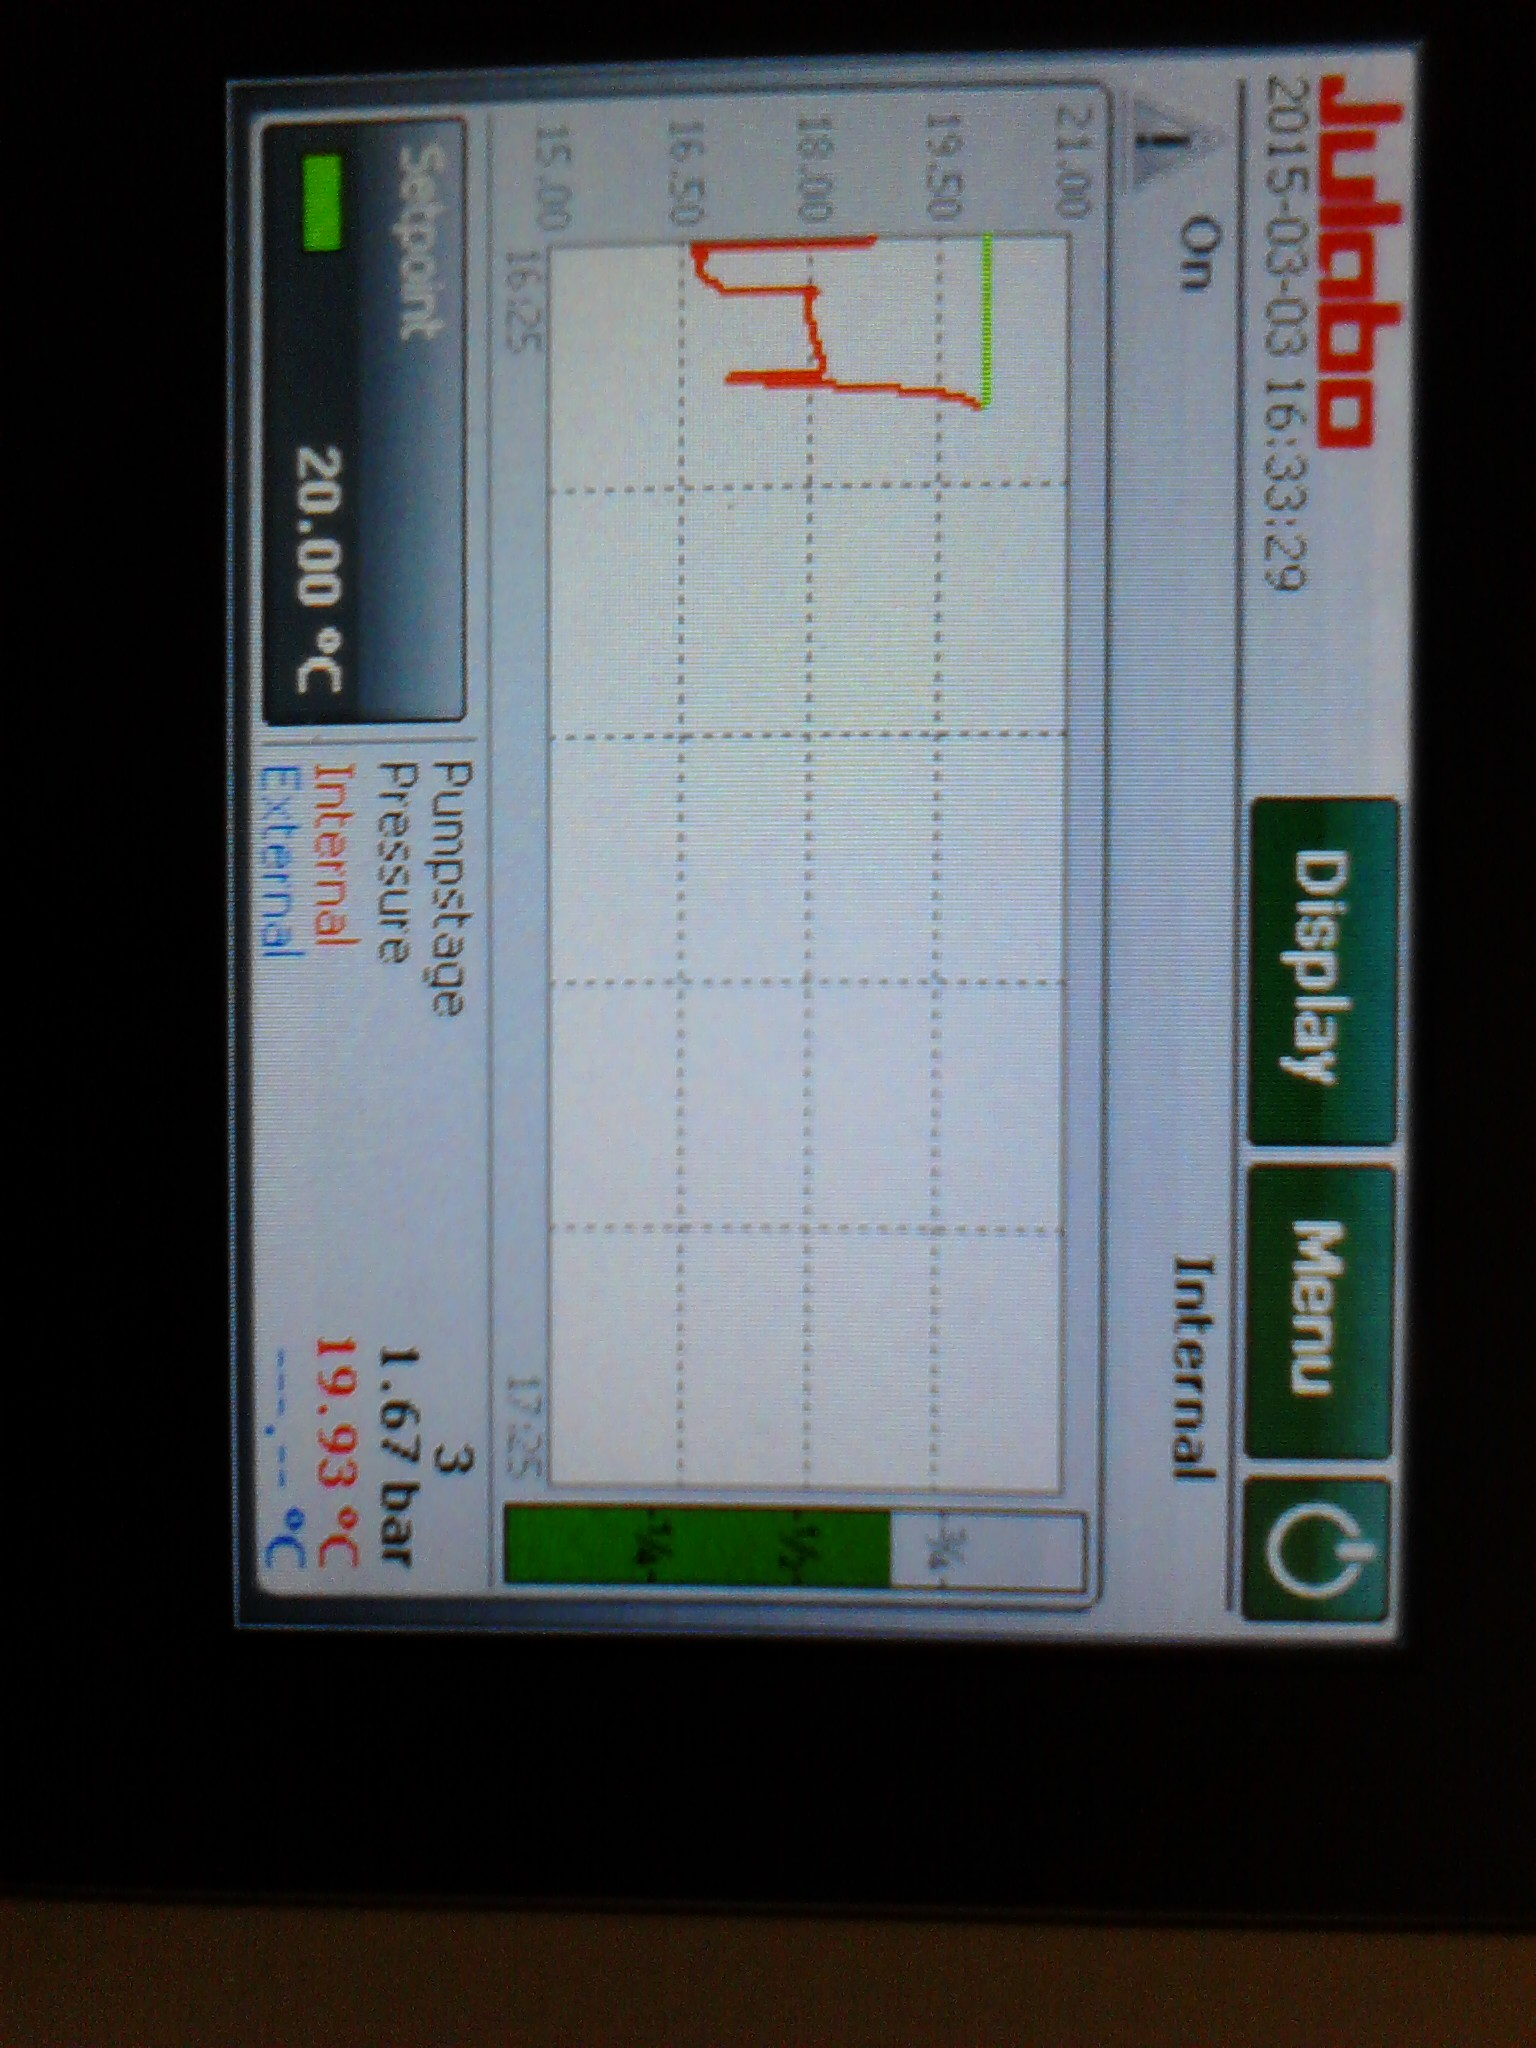
\includegraphics[angle=90,width=6cm]{figures/chiller_level6}
    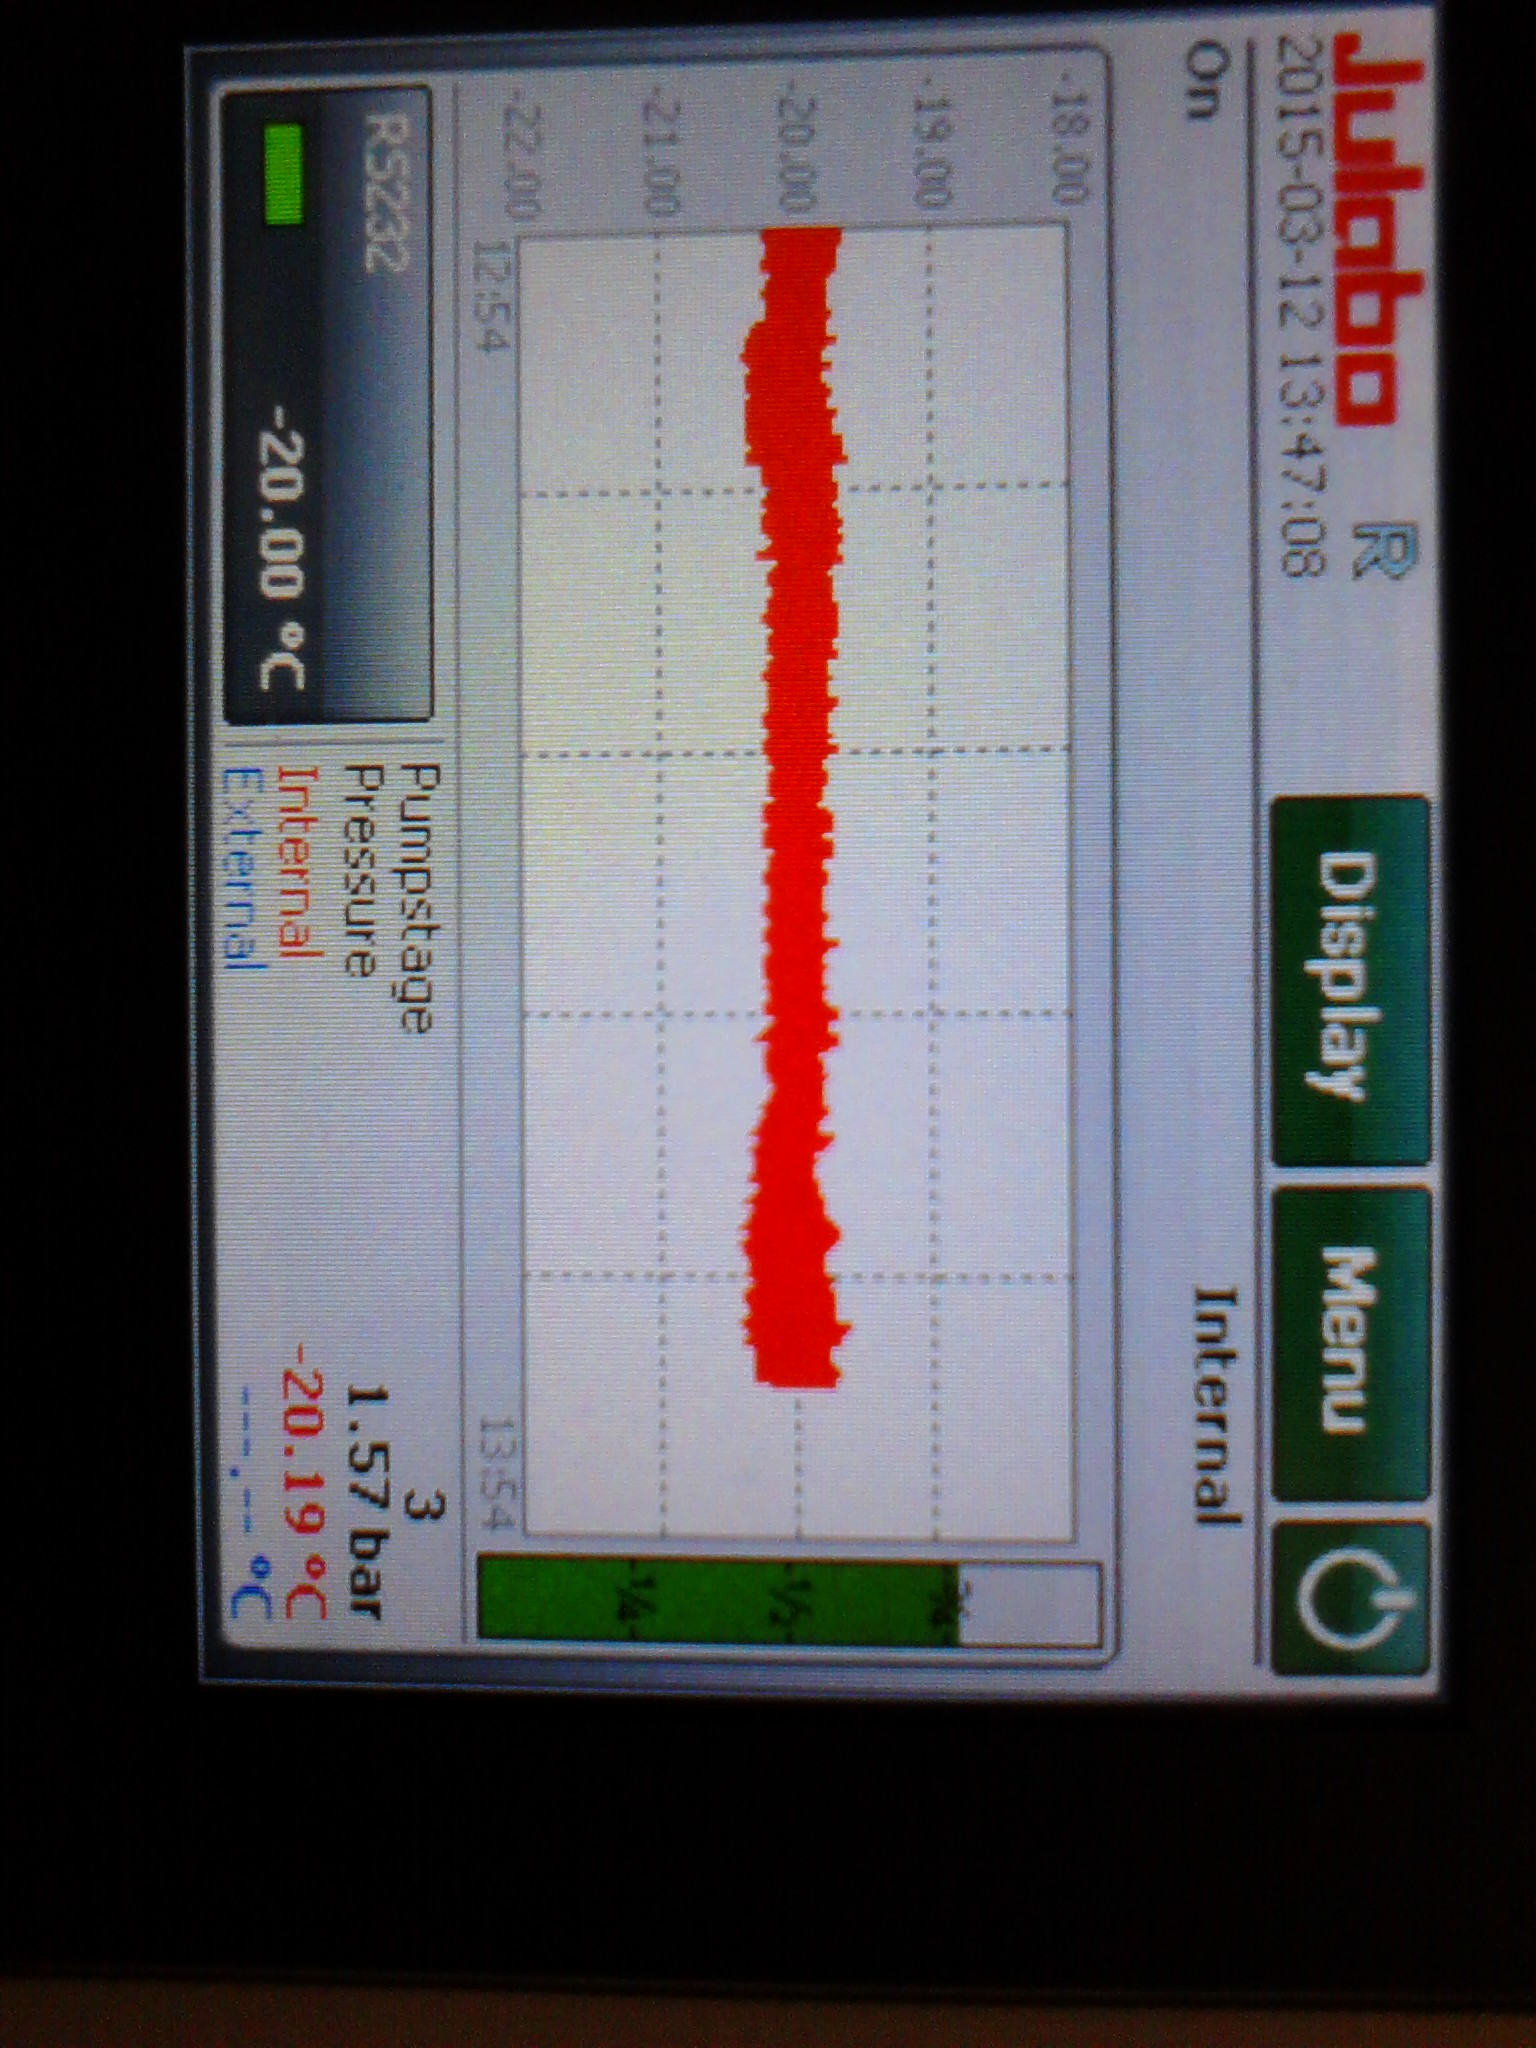
\includegraphics[angle=90,width=6cm]{figures/chiller_level7}
    \caption{Steps of the SVT chiller level indicator (green/yellow bar on right - it may be necessary to push the green ``Display'' button at the top to get to this view). Level 1 (first image) is the lowest level at which the chiller will continue to run, with a low level warning alarm. Levels 2--7 are levels for normal operation. Level 8 (not shown) will cause a high level warning alarm, but the chiller will continue to run. \label{fig:svt_chiller_level}}
\end{figure}

\subsection{Response to unexpected chiller trip}
\label{sec:proc_cooling_chillertrip}

\begin{enumerate}
    \item Look at the EPICS screens for the PLC. Check the alarm status fields for any PLC alarms. Also look at the software interlock screen and check the interlock status fields for any interlock faults. Call the SVT expert with the list of alarms.
    \item If the expert tells you to restart the chiller: Disable all PLC alarms that have tripped. Bypass and reset all software interlocks that have tripped. Start the chiller from its EPICS screen. As alarms clear, re-enable all alarms and interlocks that you disabled. If any alarm does not clear, call the SVT expert.
\end{enumerate}



\end{document}
